\documentclass[12pt,letterpaper]{report}
\usepackage{natbib}
\usepackage{geometry}
%\usepackage{fancyheadings} fancyheadings is obsolete: replaced by fancyhdr. JL
\usepackage{fancyhdr}
\usepackage{afterpage}
\usepackage{graphicx}
\usepackage{amsmath,amssymb,amsbsy}
\usepackage{dcolumn,array}
\usepackage{tocloft}
\usepackage{asudis}
\usepackage{acronym}
\usepackage{listings}
\usepackage{color}


\acrodef{sc}[SC]{Smart Contract}
\acrodef{dapp}[DApp]{Decentralized Application}
\acrodef{ct}[CT]{Challenge Task}

\definecolor{lightgray}{rgb}{.8,.8,.8}
\definecolor{darkgray}{rgb}{.6,.6,.6}
\definecolor{purple}{rgb}{0.65, 0.12, 0.82}
\definecolor{orange}{rgb}{1.0, 0.41, 0.01}
\definecolor{forestgreen}{rgb}{0.04, 0.39, 0.13}

\lstdefinelanguage{JavaScript}{
	keywords={typeof, new, true, false, catch, function, return, null, catch, switch, var, if, in, while, do, else, case, break, event, uint, adress, bytes32, public, storage, memory, string, bool, , view, return, for},
	keywordstyle=\color{orange}\bfseries,
	ndkeywords={class, export, boolean, throw, implements, import, this},
	ndkeywordstyle=\color{darkgray}\bfseries,
	identifierstyle=\color{black},
	sensitive=false,
	comment=[l]{//},
	morecomment=[s]{/*}{*/},
	commentstyle=\color{purple}\ttfamily,
	stringstyle=\color{forestgreen}\ttfamily,
	morestring=[b]',
	morestring=[b]"
}

\lstset{
	language=JavaScript,
	backgroundcolor=\color{lightgray},
	extendedchars=true,
	basicstyle=\tiny\ttfamily\linespread{0},
	showstringspaces=false,
	showspaces=false,
	numbers=left,
	numberstyle=\scriptsize,
	numbersep=1pt,
	tabsize=1,
	breaklines=true,
	showtabs=false,
	captionpos=b
}

\begin{document}
%-----------------------front matter
\pagenumbering{roman}
\title{Challenge Task 2018}
\subtitle{Implementation of a Decentralized Application Tic Tac Toe}
\paperType{Dissertation}
\chair{Departements of Informatics - Communication Systems Group}
\memberOne{Lucas Pelloni, 13-722-038}
\memberTwo{Severin Wullschleger 13-715-081}
\memberThree{Andreas Schaufelbühl, 12-918-843}


\maketitle
\doublespace
\tableofcontents
\newpage
%-----------------------body
\doublespace
\pagenumbering{arabic}

\chapter{Introduction}\label{ch:introduction}
%introduce to the task and idea
This years \ac{ct} is to implement a \ac{dapp}  running in the Ethereum blockchain. The goal of the application is a playable Tic-Tac-Toe\footnote{https://en.wikipedia.org/wiki/Tic-tac-toe} game, which also includes a betting system, all embedded in a \ac{sc}.
\\\\
%Introduce more our project here

Chapter \ref{ch:technologies} gives an overview and short explanation of the technologies we use in order to implement the \ac{ct}.\\
In Chapter \ref{ch:implementation} we show the actual implementation of the game. It starts by explaining and showing our project structure. Also we give walk-through of the different processes of playing a game and betting on games.\\
The problems and challenges occurred within our project are discussed in Chapter \ref{ch:discussion}. Additionally we also describe our open task and goals for the future concerning this project.
\chapter{Technologies}
%which technologies are used and why

\chapter{Implementation of the game}\label{ch:implementation}
\section{The Smart Contract}
\noindent The diagram in Figure\ref{fig:sc_uml}  shows a detail structure explaining the modelling of our \ac{sc}. \\
\begin{figure}[ht]
	\begin{center}
		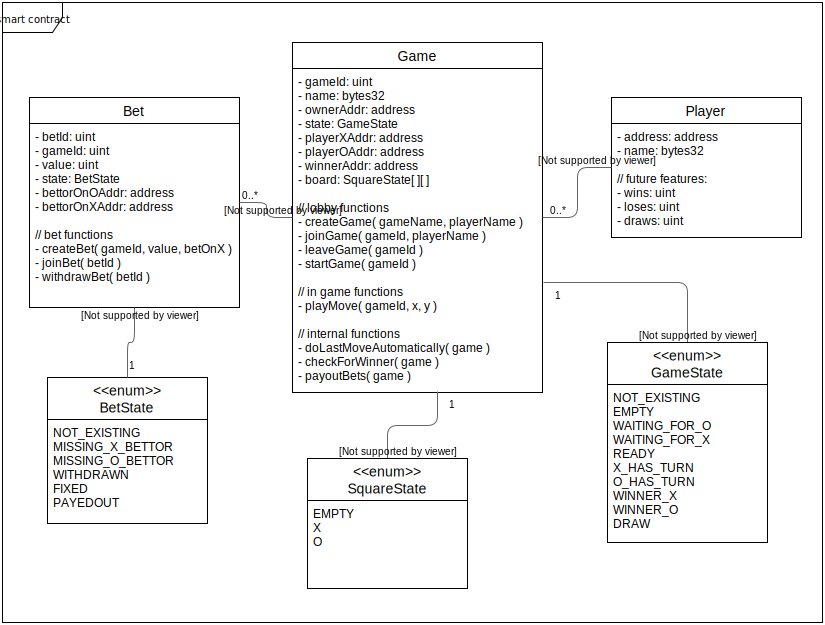
\includegraphics[scale=0.22]{res/sc_uml}
	\end{center}
	\caption{Structure of the \ac{sc}}
	\label{fig:sc_uml}
\end{figure}\newline
\noindent The \ac{sc} can hold multiple games, which always contain one board and two players. Every time a user opens up a new Game, he automatically gets assigned as one of the playing party. Now the Game state is automatically set to 'WAITING\_FOR\_X'. As soon as a second player chooses to enter a open game, the game-owner can start the game, which changes the state to 'X\_HAS\_TURN' as the game has now started and the guest player has to do his first move.\\\\
All Bets contain a game-id pointing to a game which the bet is referencing on it. The user who creates a bet chooses the game and the amount of token he wants to bet with and pays it into the \ac{sc}. Is there an opponent bettor joining the bet, the state changes to 'FIXED'.\\
If the game finds an end, the state of it changes to either 'WINNER\_X', 'WINNER\_O' or 'DRAW', which activates the function 'payout' ,triggering all bets referencing to this particular game. So the bets will change the state to 'PAYOUT' and user will get paid according to their betting.\\ 
Three functions of the \ac{sc} we show here, to discuss in detail the implementation and structure of the \ac{sc}:\\





%logic and modell

\subsection{Play Move Function}\label{subsec:move}
	\begin{lstlisting}[caption={Play Move Function on the Smart Contract}, label={lst:move},language=JavaScript,escapechar=|]
event MoveMade(bool success, uint gameId, GameState state, uint x, uint y, string symbol);|\label{line:event}| 
function playMove(uint gameId, uint x, uint y) public { |\label{line:param}| 
	Game storage game = games[gameId];|\label{line:mapping}|
		    
	require(game.state >= GameState.X_HAS_TURN, "The game is not started yet.");
	require(game.state < GameState.WINNER_X, "The game is already finished.");
		    
	game.moveCounter += 1;
		    
	if (game.state == GameState.X_HAS_TURN) {
		require(game.playerXAddr == msg.sender
			|| game.moveCounter == boardSize * boardSize// last move made 	automatically
			, "Sender not equal player X");
		require(game.board[y][x] == SquareState.EMPTY
		,"Move not possible because the square is not empty.");
		    
		game.board[y][x] = SquareState.X;|\label{line:boardX}|
		game.state = GameState.O_HAS_TURN;
		checkForWinner(x, y, gameId, game.playerXAddr);|\label{line:winnerX}|
		    
		emit MoveMade(true, gameId, game.state, x, y, "X");|\label{line:emit1}|
	}
	else {
		require(game.playerOAddr == msg.sender
			|| game.moveCounter == boardSize * boardSize      // last move made automatically
			, "Sender not equal player O");
		require(game.board[y][x] == SquareState.EMPTY
			, "Move not possible because the square is not empty.");
		    
		game.board[y][x] = SquareState.O;|\label{line:boardO}|
		game.state = GameState.X_HAS_TURN;
		checkForWinner(x, y, gameId, game.playerOAddr);|\label{line:winnerO}|
		    
		emit MoveMade(true, gameId, game.state, x, y, "O");|\label{line:emit2}|
	}
	if (game.moveCounter == boardSize*boardSize - 1 && game.state < GameState.WINNER_X) {
		doLastMoveAutomatically(game);|\label{line:lastMove}|
	}
}
\end{lstlisting}
The code of the playMove function is shown in Listing \ref{lst:move}. This gets called when a player clicks on a tile in order to make his move.The game id is send as an parameter (line \ref{line:param}). With this id the corresponding game object can be called through a mapping (line \ref{line:mapping})  It adds the players symbol into the specific location within the game-board firstly (line \ref{line:boardX} and \ref{line:boardO}). Afterwards it calls the 'checkForWinner' function (line \ref{line:winnerX} and \ref{line:winnerO}). The event MoveMade (line \ref{line:event}) is triggered returning the user an confirmation of the move (line \ref{line:emit1} and \ref{line:emit2}). There is also an an auto completion for the last move if there is no winner set yet (line \ref{line:lastMove}).



\subsection{Check for Winner}\label{subsec:check}
\begin{lstlisting}[caption={Check for Winner Function on the Smart Contract}, label={lst:check},language=JavaScript,escapechar=|]
function checkForWinner(uint x, uint y, uint gameId, address currentPlayer) private {
	Game storage game = games[gameId];
	
	//is winning already possible?
	if (game.moveCounter < 2 * boardSize - 1) |\label{line2:win}|
		return;
	}
	
	SquareState symbol = game.board[y][x];
	
	//check column
	for (uint i = 0; i < boardSize; i++) { |\label{line2:check1}|
		if (game.board[i][x] != symbol) {
			break;
		}
		else if (i == (boardSize - 1)) {
			game.winnerAddr = currentPlayer;
			game.state = getGameState(symbol);
			payoutBets(game.gameId); |\label{line2:pay1}|
			return;
		}
	}
	
	//check row
	for (i = 0; i < boardSize; i++) {	|\label{line2:check2}|
		if (game.board[y][i] != symbol) {
			break;
		}
		else if (i == (boardSize - 1)) {
			game.winnerAddr = currentPlayer;
			game.state = getGameState(symbol);
			payoutBets(game.gameId); |\label{line2:pay2}|
			return;
		}
	}
	
	//check diagonal: (x-y) 0-0, 1-1, 2-2 
	if (x == y) {					|\label{line2:check3}|
		for (i = 0; i < boardSize; i++) {
			if (game.board[i][i] != symbol) {
				break;
			}
			else if (i == (boardSize - 1)) {
				game.winnerAddr = currentPlayer;
				game.state = getGameState(symbol);
				payoutBets(game.gameId); |\label{line2:pay3}|
				return;
			}
		}
	}
	
	// check antidiagonal: (x-y) 2-0, 1-1, 0-2
	if (x + y == (boardSize - 1)) {			|\label{line2:check4}|
		for (i = 0; i < boardSize; i++) {
			if (game.board[i][boardSize - 1 - i] != symbol) {
				break;
			}
			else if (i == (boardSize - 1)) {
				game.winnerAddr = currentPlayer;
				game.state = getGameState(symbol);
				payoutBets(game.gameId);|\label{line2:pay4}|
				return;
			}
		}
	}
	//check for draw
	if (game.moveCounter == boardSize * boardSize) { |\label{line2:check5}|
		game.state = GameState.DRAW;
		payoutBets(game.gameId); |\label{line2:pay5}|
	}
}
\end{lstlisting}

The logic for the evaluating the winner function is shown in Listing \ref{lst:check}. The function stops if the number of moves played are not enough to possibly have a winner (line \ref{line2:win}). After it goes through all possible combination of winning and checks if there are the same symbol within a line (line \ref{line2:check1}, \ref{line2:check2}, \ref{line2:check3} and \ref{line2:check4}). If it does not found any winning line it checks at last for a draw (line \ref{line2:check5}). Is there a winning line found or the game is a draw, the payout function gets called (line \ref{line2:pay1}, \ref{line2:pay2}, \ref{line2:pay3}, \ref{line2:pay4} and \ref{line2:pay5}).
\subsection{Payout}\label{subsec:payout}
\begin{lstlisting}[caption={Payout Function on the Smart Contract}, label={lst:payout},language=JavaScript,escapechar=|]
function payoutBets(uint gameId) internal {
	for (uint i = 0; i < openBetIds.length; i++) |\label{line3:loop1}|
		Bet storage iBet = bets[openBetIds[i]];
   
		if (iBet.gameId == gameId) { |\label{line3:loop2}|
			if (iBet.state == BetState.FIXED) {
   
				// bettorOnX wins
				if (games[gameId].state == GameState.WINNER_X) {
					(iBet.bettorOnXAddr).transfer(SafeMath.mul(2, iBet.value)); |\label{line3:safe1}|
   
				// bettorOnO wins
				} else if (games[gameId].state == GameState.WINNER_O) {
					(iBet.bettorOnOAddr).transfer(SafeMath.mul(2, iBet.value)); |\label{line3:safe2}|
   
				// draw
				} else {
					(iBet.bettorOnOAddr).transfer(iBet.value);
					(iBet.bettorOnXAddr).transfer(iBet.value);
				}
				iBet.state = BetState.PAYEDOUT;
			}
   
			// handle not fixed bets: transfer value back to owner
			if (iBet.state == BetState.MISSING_O_BETTOR) { |\label{line3:back1}|
			   (iBet.bettorOnXAddr).transfer(iBet.value);
			   iBet.state = BetState.WITHDRAWN;
			}
			if (iBet.state == BetState.MISSING_X_BETTOR) {
				(iBet.bettorOnOAddr).transfer(iBet.value);
				iBet.state = BetState.WITHDRAWN;
			} |\label{line3:back2}|
		}
	}
}
\end{lstlisting}
If there is a winner or a draw the tokens reserved for the particular game get paid out with the payout method describe in Listing \ref{lst:payout}. As it can have multiple bets on one game the function runs through all bets checking if they are referencing on the finished game (line \ref{line3:loop1}-\ref{line3:loop2}). SafeMath is used for the payout to assure the amount is correct and prevent overflow (line \ref{line3:safe1} and \ref{line3:safe2}). When a bettor has not found an opponent to go along with his bet, the function pays back the value to the origin bettor (line \ref{line3:back1}-\ref{line3:back2}). 
\chapter{Discusion}\label{ch:discussion}
\section{Challenges and Problems}
\section{Future work}
%logic and modell
\include{chapter5}
\include{chapter6}
%-----------------------back matter
{\singlespace
% Making the references a "part" rather than a chapter gets it indented at
% level -1 according to the chart: top of page 4 of the document at
% ftp://tug.ctan.org/pub/tex-archive/macros/latex/contrib/tocloft/tocloft.pdf
\addcontentsline{toc}{part}{REFERENCES}
\bibliographystyle{asudis}
\bibliography{dis}}
\renewcommand{\chaptername}{APPENDIX}
\include{vita}

\end{document}

